\documentclass{article}
\usepackage[utf8]{inputenc}


\title{\textbf{PROVA INTERCORSO A.D.C}}
\author{Pasquale Del Prete}
\date{17/11/2020}


\usepackage{natbib}
\usepackage{graphicx}

\begin{document}
\maketitle


\section{\textbf{DOMANDA N.1}\textit{ differenze tra memorie}}
La teoria delle stringhe prese le \textbf{mosse da un articolo} che Gabriele Veneziano scrisse per spiegare il comportamento degli adroni. ... Nessun semplice modello adronico, ad esempio quello che li considera composti da una serie di particelle \textbf{più piccole} legate da un qualche tipo di forza, spiega tali relazioni.
\section{\textbf{RISPOSTA 1 : }}
\textbf{LA MEMORIA CACHE} è una tipo di memoria molto veloce
\begin{figure}[h!]
\centering
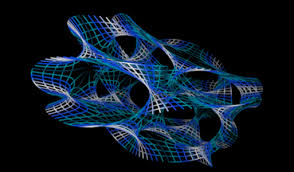
\includegraphics[scale=1.0]{teoria delle stringhe esempio overleaf.jpg}
\caption{Teoria Delle stringhe}
\label{fig:Teoria Delle Stringhe}
\end{figure}

\section{Formula Della Teoria Delle Stringhe}
la formula e molto complicata ti consiglio di adare a vederk su wiki


\end{document}